\chapter{Introduction}

Software is increasingly complex with many interactions with other software
and the operating system.
The complex interactions make the software ecosystem hard to understand.
Without proper understanding,
it is difficult to configure/maintain software and to fix problems.
The complexity also increases the attack surface, which measures the
bugs or features exploitable by malicious attacks.
Operating system monitoring is an effective way to understand these
interactions.
Monitoring can also verify correctly running software or discover
unexpected behaviours such as performance problems or malicious attacks.
However, there are challenges with system monitoring.
The interactions may not be well defined or understandable,
especially when the source code or proper documentation is not available.
The monitoring system itself can inevitably affect the monitored system
in an undesirable way.
The monitoring system cannot be trusted if the host on which it
runs is compromised.
Lastly, the huge amount of information produced is hard to maintain and
analyze.

This introductory chapter is organized as follows.
Section~\ref{sec:motivation} motivates the research on operating system monitoring.
% Section~\ref{sec:win-issue} discusses the some background and difficulties related
% to system monitoring in the Windows operating system.
Section~\ref{sec:contribution} summarizes the contributions of our research.

\section{Motivation}
\label{sec:motivation}

\TODO{...}

\section{Contribution}
\label{sec:contribution}

\begin{figure}[htb]
\centering
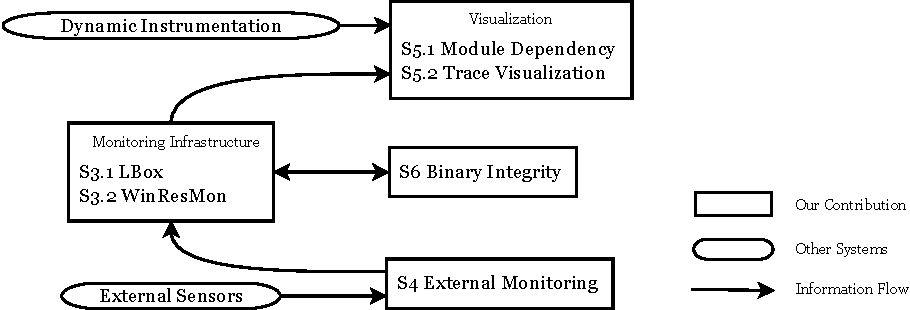
\includegraphics[width=0.8\textwidth]{overview.pdf}
\caption{Overview of the contributions}
\label{fig:overview}
\end{figure}

\TODO{3 parts: monitoring (lbox, winresmon);
software understanding (depvis, lviz);
system security (sensor, binauth)}
